%!TeX spellcheck = de_DE

\providecommand{\additionalOptionsForClass}{}
\documentclass[
  accentcolor=tud1c,	% Color theme for TUD corporate design
  colorbacktitle,		% Titlepage has colored background for title area
  inverttitle,			% Font color of title on titlepage is inverted
  \additionalOptionsForClass
  %german%,
  %twoside
]{tudexercise}

\parindent1em
%\parskip2ex

\usepackage[ngerman]{babel}
\usepackage[utf8]{inputenc}
\usepackage{listings}
\usepackage{booktabs}
\usepackage{amsmath}
\usepackage{algorithm2e}
\usepackage{hyperref}
\usepackage{xspace}
\usepackage{tabularx}
\usepackage{tikz}
\usepackage{cleveref}
\usepackage{numprint}
\usepackage{paralist}
\usepackage{verbatim}
\usepackage{tocloft} % for manipulating the table of contents

\usetikzlibrary{shapes}
\usetikzlibrary{calc}
\usetikzlibrary{arrows}
\usetikzlibrary{decorations}

\usepackage{pifont}
\newcommand{\cmark}{\ding{51}\xspace}%
\newcommand{\xmark}{\ding{55}\xspace}%

\usepackage{todonotes}
%\usepackage[disable]{todonotes} % Use this line to hide all todos

\definecolor{commentgreen}{RGB}{50,127,50}
\lstloadlanguages{C++,[gnu]make}
\lstset{language=C++}
\lstset{captionpos=b}
\lstset{tabsize=3}
\lstset{breaklines=true}
\lstset{basicstyle=\ttfamily}
\lstset{columns=flexible}
\lstset{keywordstyle=\color{purple}}
\lstset{stringstyle=\color{blue}}
\lstset{commentstyle=\color{commentgreen}}
\lstset{otherkeywords=\#include}
\lstset{showstringspaces=false}
\lstset{keepspaces=true}
\lstset{xleftmargin=1cm}
\lstset{literate=%
	{Ö}{{\"O}}1
	{Ä}{{\"A}}1
	{Ü}{{\"U}}1
	{ß}{{\ss}}2
	{ü}{{\"u}}1
	{ä}{{\"a}}1
	{ö}{{\"o}}1
	{'}{{\textquotesingle}}1
}

\lstnewenvironment{lstmake} %
{\lstset{language=[gnu]make}} %
{}


\newcommand{\superscript}[1]{\ensuremath{^{\textrm{#1}}}}
\newcommand{\subscript}[1]{\ensuremath{_{\textrm{#1}}}}

\newcommand{\setHeader}[1]{
\providecommand{\examheadertitle}{TODO: Titel einbinden}
\renewcommand{\examheadertitle}{#1}
\begin{examheader}
    \examheadertitle
\end{examheader}
}

\newcommand{\hints}[1]{
\paragraph*{Hinweise}
	\begin{itemize}
		\setlength{\itemsep}{0pt}
		#1
	\end{itemize}
}

\newcommand{\optional}{\xspace(optional)}
\newcommand{\experimental}{\xspace(experimentell)}

\usepackage{fancybox}
\newcommand{\optionaltextbox}{
	\bigskip
	\begin{center}
		\ovalbox{\parbox{0.98\textwidth}{Die Klausur kann ohne diese Aufgabe bestanden werden. Wir empfehlen aber sie trotzdem zu bearbeiten.}}
	\end{center}
}
\newcommand{\experimentaltextbox}{
	\bigskip
	\begin{center}
		\ovalbox{\parbox{0.98\textwidth}{Diese Aufgabe wurde neu erstellt und kann noch Fehler und Inkonsistenzen enthalten. Falls euch etwas derartiges auffällt sprecht uns bitte darauf an oder stellt es auf GitHub in den Issuetracker unter \url{https://github.com/Echtzeitsysteme/tud-cpp-exercises/issues}}}
	\end{center}
}

\newcommand{\enquote}[1]{\glqq#1\grqq\xspace}
\newcommand{\filename}[1]{\texttt{#1}}

\newcommand{\RK}[1]{\todo[]{\textbf{RK:} #1}}
\newcommand{\RKi}[1]{\todo[inline]{\textbf{RK:} #1}}

\newcommand{\ExercisePrefix}[1]{$[$#1$]$ \xspace}
\newcommand{\ExercisePrefixBasics}{\ExercisePrefix{G}}
\newcommand{\ExercisePrefixMemory}{\ExercisePrefix{S}}
\newcommand{\ExercisePrefixObjectOrientation}{\ExercisePrefix{O}}
\newcommand{\ExercisePrefixAdvanced}{\ExercisePrefix{F}}
\newcommand{\ExercisePrefixEmbeddedC}{\ExercisePrefix{C}}
\newcommand{\ExercisePrefixElevator}{\ExercisePrefix{A}}
\newcommand{\ExercisePrefixAdditionalInformation}{\ExercisePrefix{Z}}

\title{Übung zum\linebreak[1]C/C++-Praktikum\linebreak[1] Fachgebiet Echtzeitsysteme\linebreak[1]\linebreak[1] Speicherverwaltung}

\setcounter{section}{0}

%optional parameters to speed up build (increases pdf file size)
%\pdfcompresslevel=0
%\pdfobjcompresslevel=0
\begin{document}

\maketitle

\setcounter{tocdepth}{1}
\setlength\cftsecnumwidth{10em}
\setlength\cftbeforesecskip{.1em} % line skip between sections ("sec")

\setHeader{Aufgaben zur Speicherverwaltung in C++}

\section{\ExercisePrefixMemory Zeiger und Referenzen Grundlagen}
In dieser Aufgabe sollst du den Umgang mit Zeigern (\emph{Pointer}) und Referenzen erlernen.
Diese erlauben es zum Beispiel Werte zwischen Funktionen auszutauschen, ohne eine Kopie der zu übermittelnden Daten zu erzeugen.
Anstelle dessen kann ein (vergleichsweise kleiner) Zeiger auf einen Speicherbereich übergeben werden.
Alternativ kann auch eine Referenz auf eine Variable übergeben werden, welche intern ähnlich wie ein Zeiger gehandhabt wird.

\subsection{Experimente}
Experimentiere mit Zeigern, Adressen und Referenzen. Als Ausgangsbasis kann folgendes Programmfragment dienen.
Fülle danach die untenstehende Skizze aus, um dir klarzumachen, wie Variablen und ihre Speicherabbilder zusammenhängen.

\lstinputlisting{02_memory/problems/listings/pointers_intro.cpp}

\paragraph{Speicherabbild}
Wir nehmen an, dass Speicheradressen immer 4 Byte (= 32 Bit) breit sind. 
Trage nun die auftretenden Variablen \lstinline{intVal} und \lstinline{pIntVal} in das folgende Speicherabbild ein. Orientiere dich dabei an der Vorlesung (Folien 69 und 70) und trage folgende Dinge ein:
\begin{itemize}
	\item Typ, Name und Wert jeder Variablen
	\item Speicheradressen in Bytes
	\item Der Wert, der an der jeweiligen Speicheradresse steht.
\end{itemize}

\begin{center}
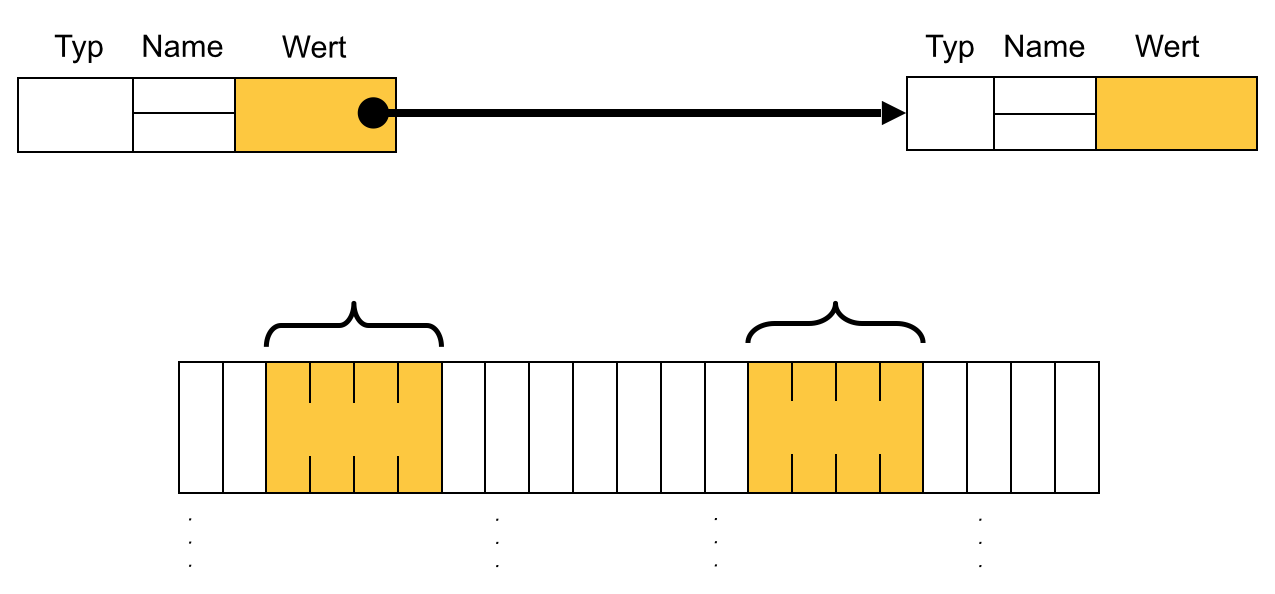
\includegraphics[width=.9\textwidth]{02_memory/figures/memory_image.png}
\end{center}

\hints{
	\item Die Speicheradressen kannst du frei wählen, der Pointer sollte aber natürlich auf die entsprechend gewählte Adresse zeigen.
}

\subsection{Bedeutung verstehen}
Versuche die Bedeutung folgender Ausdrücke zu verstehen.
Welche Regelmäßigkeiten stellst du fest?

\begin{minipage}{\linewidth}
\lstinputlisting{02_memory/problems/listings/pointers_intro_advanced.cpp}
\end{minipage}

\hints{
	\item Gehe dabei von rechts nach links vor.
}

\subsection{Gültigkeit}
Warum sind folgende Ausdrücke ungültig, sinnlos oder sogar gefährlich?

\vbox{ %fixes empty page
\lstinputlisting{02_memory/problems/listings/pointers_intro_validity.cpp}
}

\hints{
	\item Finde heraus, welchen Typ der Ausdruck hätte haben müssen.
	\item Nur tatsächlich angelegte Variablen haben Adressen. Ausdrücke wie a + b oder direkt kodierte Zahlenliterale wie 42 haben keine Adresse.
}

\subsection{Variablentausch}
Schreibe eine Funktion \lstinline{swap}, die zwei \lstinline{int}-Variablen miteinander vertauscht.
Probiere dabei beide möglichen Übergabevarianten (per Referenz, per Pointer) aus.
Was würde passieren, wenn man die Variablen stattdessen per Wert übergeben würde?

\subsection{Programmanalyse}
Sieh dir folgendes Programm an.

\vbox{ %fixes empty page
\lstinputlisting{02_memory/problems/listings/pointers_programm.cpp}
}

Welche Adressen werden übereinstimmen, welche werden sich unterscheiden?
Führe das Programm aus.
Hast du diese Ausgabe erwartet?

\subsection{Const Correctness}

In dieser Aufgabe setzt du dich mit der Bedeutung des Schlüsselworts \lstinline{const} im Kontext von Pointern auseinander.

Versuche für jede der Variablen im folgenden Code je eine \emph{Verwendung} zu finden, die  
\begin{itemize}
\item gültig ist (= fehlerfrei kompiliert) und
\item nicht gültig ist (= einen Compiler-Fehler wirft).
\end{itemize}


Was ist jeweils der Grund?
Welche Pointer verhalten sich gleich?

\lstinputlisting{02_memory/problems/listings/pointers_behavior.cpp}

\paragraph{Mehrstufige Pointer}

Versuche nun das Gleiche mit den folgenden mehrstufigen Pointern.

\lstinputlisting{02_memory/problems/listings/pointers_multi.cpp}

\subsection{Übergabewerte}
In der letzten Aufgabe direkt zu Pointern geht es darum, das gerade erlangte Verständnis über Pointer und Referenzen zu festigen und zu kontrollieren.
In Tabelle \ref{table:uebergabewerte} sind in der ersten Spalte Funktionen mit verschiedenen Parametern gegeben.
In der ersten Zeile findest du verschiedene Variablentypen.
Deine Aufgabe ist es nun, zu den verschiedenen Funktionen die passenden Parameter aus den Variablen herzustellen.
Falls eine Variable nicht ohne großartige Konversationen verwendet werden kann trage bitte ein \xmark ein. \\\\
Als Beispiel dient hierfür die erste Zeile. 

\begin{table}[h]
    \centering

    \newcolumntype{b}{X}
    \newcolumntype{s}{>{\hsize=.6\hsize}X}

    \begin{tabularx}{\textwidth}{b *5{| >{\centering\arraybackslash}s}@{}} 
		& \mbox{\lstinline!int i!} & \mbox{\lstinline!int *j!} & \mbox{\lstinline!int const *const k!} & \mbox{\lstinline!int **l!} & \mbox{\lstinline!const int *m!} \\ \hline
		\mbox{\lstinline!op1(int *)!}          & \mbox{\lstinline!&i!} & \mbox{\lstinline!j!} & \xmark & \mbox{\lstinline!*l!} & \xmark \\ \hline
		\mbox{\lstinline!op2(int)!}            & & & & & \\ \hline
		\mbox{\lstinline!op3(int &)!}         & & & & & \\ \hline
		\mbox{\lstinline!op4(const int **)!}   & & & & & 
    \end{tabularx}
    \caption{Tabelle für \emph{Übergabewerte} Aufgabe}
    \label{table:uebergabewerte}
\end{table}

\newpage
\section{Arrays und Zeigerarithmetik}
Arrays sind zusammenhängende Speicherbereiche, die mehrere Variablen von gleichem Typ speichern können.
Arrays werden in C++ folgendermaßen angelegt: \lstinline{<Typ> <name>[<Größe>];}, zum Beispiel:

\lstinputlisting{02_memory/problems/listings/arrays_intro.cpp}

Falls das Array global ist, muss die Größe eine konstante Zahl sein, falls das Array in einer Funktion auf dem Stack angelegt wurde, kann die Größe auch durch eine Variable vorgegeben werden.
Auf jeden Fall bleibt diese während der Existenz des Arrays konstant und kann sich nach dem Anlegen nicht mehr ändern.

Ein Array kann direkt bei der Deklaration initialisiert werden:

\lstinputlisting{02_memory/problems/listings/arrays_example.cpp}

Man kann die Größe optional auch weglassen, in diesem Fall wird sie der Compiler anhand der angegebenen Elemente selbst ermitteln.

Man kann auf die einzelnen Elemente des Arrays wie gewohnt über \textbf{arr[i]} zugreifen.

Arrays und Zeiger sind in C++ stark miteinander verwandt.
So ist der \textbf{Bezeichner} des Arrays gleichzeitig die \textbf{Adresse des ersten Elements}.
Somit kann man sowohl durch \textbf{*arr} als auch durch \textbf{arr[0]} auf das erste Element zugreifen.
Analog dazu kann man auch einen Zeiger auf das erste Element anlegen:

\lstinputlisting{02_memory/problems/listings/arrays_pointer.cpp}

Da die Elemente eines Array direkt hintereinander stehen, kann man den Zeiger inkrementieren, um zum  nächsten Element zu gelangen (sogenannte Pointerarithmetik).
Beispiel:

\lstinputlisting{02_memory/problems/listings/arrays_inc.cpp}

Somit kann man auf beliebige Elemente des Array über den Zeiger zugreifen:

\lstinputlisting{02_memory/problems/listings/arrays_pointer_inc.cpp}

Tatsächlich ist \textbf{*(p+i)} in \textbf{jeder Hinsicht äquivalent} zu \textbf{p[i]}.
Das bedeutet, dass man sowohl auf das i-te Element eines Arrays über \textbf{*(arr + i)} zugreifen kann als auch über \textbf{pointer[i]} auf das Element, auf welches der Zeiger \lstinline{pointer+i} zeigt!

In C++ findet keine automatische Bereichsprüfung bei Arrayzugriffen statt.
Du bist als Programmierer selbst dafür verantwortlich, dass niemals auf ein Element außerhalb der Array-Grenze zugegriffen wird.
Falls doch, kann es zu Programmabstürzen oder unerwünschten Effekten wie Buffer-Overflows kommen, die ein erhebliches Sicherheitsrisiko darstellen.
Bevorzuge deshalb Container-Klassen wie \lstinline{std::vector} (oder \lstinline{std::array} ab C++11) aus der Standardbibliothek anstelle von \glqq rohen\grqq{} Arrays.
Beachte außerdem, dass der \lstinline{delete[]}-Operator zwar das Array löscht, den Zeiger jedoch \textbf{nicht} auf \lstinline{NULL} setzt.
Dabei entsteht ein \emph{Dangling Pointer}, welcher dazu führen kann, dass später im Programm auf Speicherstellen zugegriffen wird, die nicht reserviert sind.
Setze deshalb Zeiger nach einem \lstinline{delete}/\lstinline{delete[]} sofort auf \lstinline{NULL}, um Speicherfehler zu vermeiden.

Um die Größe eines Arrays zu ermitteln, kannst du den \lstinline{sizeof()}-Operator benutzen.
Dieser gibt generell die Anzahl der Bytes an, die eine Variable verbraucht.
Da einzelne Array-Elemente größer als ein Byte sein können, muss die Gesamtgröße des Arrays durch die Größe eines Elements geteilt werden, um auf die Anzahl der Elemente zu kommen.

\lstinputlisting{02_memory/problems/listings/arrays_sizeof.cpp}

Beachte, dass \lstinline{sizeof()} \textbf{nicht} dazu verwendet werden kann, um die Größe des Arrays herauszufinden, auf die ein Zeiger zeigt.
In diesem Fall wird \lstinline{sizeof()} nämlich die \textbf{Größe des Zeigers} und nicht die Größe des Arrays liefern!

\lstinputlisting{02_memory/problems/listings/arrays_sizeof_pointer.cpp}

\subsection{Arrays anlegen}
Lege in der \lstinline{main}-Funktion ein \lstinline{int}-Array mit 10 Elementen an, und initialisiere es mit den Zahlen 1 bis 10.
Iteriere in einer Schleife über das Array und gib alle Elemente nacheinander aus.

\subsection{printElements implementieren}
In C und C++ kann man Arrays nicht direkt an Funktionen übergeben.
Stattdessen übergibt man einen Zeiger auf das erste Element des Arrays. Aufgrund der Äquivalenz von \textbf{*(p+i) } und \textbf{p[i]} kann man in der Funktion den Zeiger syntaktisch wie das Original-Array verwenden.

Schreibe eine Funktion, die einen \lstinline{const}-Zeiger auf das erste Element eines Arrays bekommt und alle Elemente ausgibt.
Da die Funktion nur anhand des Zeigers keine Möglichkeit hat zu wissen, wie groß das Array ist, muss die Größe des Arrays durch einen weiteren Parameter übergeben werden\footnote{Statt \lstinline{unsigned int} wird oft der Standard-Typ \lstinline{size_t} genutzt (z.B. in \lstinline{std::vector}).}:

\lstinputlisting{02_memory/problems/listings/arrays_printelems.cpp}

\subsection{Offset-basierte Ausgabe}
Wie wir vorher gesehen haben, kann man mit Zeigern auch rechnen und diese nachträglich ändern.
Anstatt mit einem Index das Array zu durchlaufen, kann man stattdessen bei jeder Iteration den Zeiger selbst inkrementieren!

\lstinputlisting{02_memory/problems/listings/arrays_iterate.cpp}

Schreibe die Funktion aus der vorherigen Aufgabe so um, dass sie einen laufenden Zeiger anstatt eines Indexes verwendet.

\subsection{Iterator-basierte Ausgabe}
Ebenso kann man auch die Arraygröße auf eine andere Weise übergeben, indem man die Adresse des Elements nach dem letzten Element angibt.
Dadurch werden Schleifen der folgenden Form möglich.

\lstinputlisting{02_memory/problems/listings/arrays_iterate_end.cpp}

möglich.
Schreibe die Funktion aus der vorherigen Aufgabe entsprechend um.
Vergiss nicht, den Zeiger als \lstinline{const} zu definieren, da Elemente nur gelesen werden.
Du kannst hier \lstinline{const} doppelt verwenden, um auch sicherzustellen, dass der \lstinline{end}-Zeiger nicht verändert wird.

\subsection{Subarrays ausgeben}
Die obige Methode, über Elemente eines Arrays zu iterieren, mag dir zunächst etwas ungewöhnlich erscheinen.
Sie hat jedoch den Vorteil, dass man anstatt des ganzen Arrays auch kleinere zusammenhängende Teile davon an Funktionen übergeben kann, indem man Zeiger auf die entsprechenden Anfangs-und Endelemente setzt.
Beispiel:

\lstinputlisting{02_memory/problems/listings/arrays_print_with_index.cpp}

Experimentiere etwas mit dieser Übergabemethode in deiner eigenen Funktion!

\subsection{Arrays auf dem Heap}
Bisher haben wir das Array auf dem Stack angelegt
Mit \textbf{new[]} kann man ein Array auf dem Heap erzeugen.
Dabei wird die Adresse des ersten Elements in einem Zeiger gespeichert.
Mittels \lstinline{delete[]} \textbf{muss} man den belegten Speicher nach Benutzung freigeben.
Beispiel:

\lstinputlisting{02_memory/problems/listings/arrays_heap.cpp}

Beachte die \textbf{[]} nach \lstinline{delete}.
Diese bewirken, dass das gesamte Array und nicht bloß das erste Element gelöscht wird.

Ein Anwendungsfall von dynamischen Arrays sind Funktionen, die ein Array von vorher unbekannter Größe zurückgeben.

Schreibe eine Funktion, die beliebig viele Zahlen von der Konsole mittels \lstinline{std::cin} einliest.
Der Benutzer soll dabei zuvor gefragt werden, wie viele Zahlen er eingeben möchte.
Speichere die Zahlen in einem dynamisch angelegten Array ab und lasse die Funktion einen Zeiger darauf zurückgeben.
Hier ist ein Beispiel wie \lstinline{std::cin} zu verwenden ist:

\lstinputlisting{02_memory/problems/listings/arrays_cin_size.cpp}

Zusätzlich zum Zeiger muss die Funktion auch die Möglichkeit haben, ihrem Aufrufer die Größe des angelegten Arrays mitzuteilen.
Füge der Funktion deshalb einen weiteren Parameter hinzu, in dem entweder per Referenz oder per Zeiger eine Variable übergeben wird, um dort die Größe abzulegen\footnote{Du merkst sicherlich schon jetzt, dass es umständlich/fehleranfällig ist, wenn man die Größe eines Arrays separat speichern und übergeben muss.}.

Gib die eingelesenen Werte auf der Konsole aus.
Vergiss nicht, am Ende den Speicher freizugeben.

\newpage
\section{Verkettete Listen}
In dieser Aufgabe wollen wir eine doppelt verkettete Liste von Integern implementieren.
Dazu brauchen wir zwei Klassen:
\lstinline{ListItem} stellt ein Element der Liste mit dessen Inhalt dar und \lstinline{List} speichert die Zeiger auf Anfangs- und Endelemente und bildet den eigentlichen Zugangspunkt für die Liste.

\begin{figure}[h]
\centering
\begin{tikzpicture}
    \def\blockdist{2}
    \def\captiondist{0.35}
    \tikzstyle{triple}=[rectangle split, rectangle split part fill={white, white, yellow}, thick, rectangle split parts=3, draw, align=center, text width=1.7cm]
    \tikzstyle{arrow}=[->, thick]

    % nodes
    \node (0) [triple] {next \nodepart{second}previous \nodepart{third} content};
    \path (0.east)+(\blockdist,0) node (1) [triple] {next \nodepart{second}previous \nodepart{third} content};
    \path (1.east)+(\blockdist,0) node (2) [triple] {next \nodepart{second}previous \nodepart{third} content};
    \path (2.east)+(\blockdist,0) node (3) [triple] {next \nodepart{second}previous \nodepart{third} content};
    \path (2.east)+(\blockdist,0) node (3) [triple] {next \nodepart{second}previous \nodepart{third} content};

    \coordinate (mid) at ($(1)!0.5!(2)$);
    \path (mid.south)+(0,-3) node (root) [triple, rectangle split part fill={white, white, white}] {first \nodepart{second}last \nodepart{third}currentSize};

    \path (0.west)+(-1.5,0) node (n1) {\textbf{NULL}};
    \path (3.25)+(1.5,0) node (n2) {\textbf{NULL}};

    % arrows
    \path[arrow] (0.25) edge (1.155);
    \path[arrow] (1.25) edge (2.155);
    \path[arrow] (2.25) edge (3.155);
    \path[arrow] (3.25) edge (n2.west);

    \path[arrow] (3) edge (2);
    \path[arrow] (2) edge (1);
    \path[arrow] (1) edge (0);
    \path[arrow] (0) edge (n1.east);

    \draw[arrow] (root.0) -| (3.south);
    \draw[arrow] (root.155) -| (0.south);

    % captions
    \path (0.north)+(0,\captiondist) node (c0) [] {\textbf{ListItem}};
    \path (1.north)+(0,\captiondist) node (c1) [] {\textbf{ListItem}};
    \path (2.north)+(0,\captiondist) node (c2) [] {\textbf{ListItem}};
    \path (3.north)+(0,\captiondist) node (c3) [] {\textbf{ListItem}};
    \path (root.north)+(0,\captiondist) node (croot) [] {\textbf{List}};
\end{tikzpicture}

\caption{Linked List}
\end{figure}

Wir werden am Tag 4 auf dieser Aufgabe aufbauen und die Liste um weitere Funktionen erweitern.
Behalte dies bitte im Hinterkopf und lösche deine Lösung nicht.
Falls du mit dieser Aufgabe bis dahin nicht fertig sein solltest, kannst du natürlich auch die Musterlösung als Ausgangspunkt nehmen.

\subsection{Klasse \lstinline{ListItem}}
Implementiere die Klasse \lstinline{ListItem}, welche die zu speichernde Zahl sowie Verweise auf das vorherige und nächste \lstinline{ListItem} als Attribute hat.
Verwende dazu Zeiger und keine Referenzen, da Referenzen nachträglich nicht mehr geändert werden können.
Auch können Referenzen nicht \lstinline{NULL} sein, was in unserem Fall nötig ist, um zu markieren, dass ein Element keine Vorgänger oder Nachfolger hat.

Der Konstruktor sollte sowohl seine eigenen \lstinline{next} und \lstinline{previous} Zeiger initialisieren, als auch die seiner Vorgänger- und Nachfolgerelemente.
Die Methode \lstinline{getContent()} soll eine Referenz auf den Inhalt zurückgeben, damit dieser durch eine Zuweisung modifiziert werden kann.

\begin{lstlisting}
class ListItem {
public:
	/**
	 * create a list item between two elements with a given given content
	 * (also modify previous->next and next->previous)
	 */
	ListItem(ListItem *prev, ListItem *next, int content);
	/**
	 * delete this list item (also change previous->next and next->previous
	 * to not point to this item anymore)
	 */
	~ListItem();				
	int & getContent();			// get a reference to the contained data
	ListItem * getNext();			// get the next list item or NULL
	ListItem * getPrevious();	// get the previous list item or NULL
private:
	ListItem *previous;		// previous item in list
	ListItem *next;			// next item in list
	int content;				// content of this list item
};
\end{lstlisting}

\subsection{Privater Copy-Konstruktor}
Unsere \lstinline{ListItem} Klasse hat einen kleinen Design-Fehler:
Da wir keinen Copy-Konstruktor definiert haben, generiert der Compiler automatisch einen.
Dieser kopiert einfach die einzelnen Attribute des Ursprungsobjekts (sogenannte ,,flache'' Kopie/Shallow Copy).
In unserem Fall ergibt das Kopieren eines \lstinline{ListItems} jedoch semantisch keinen Sinn, weil dabei ein hängendes \lstinline{ListItem} entstehen würde, welches nicht mit der Liste verknüpft ist, aber dennoch auf andere Items der Liste zeigt.

Deklariere in der Headerdatei einen \lstinline{private} Copy-Konstruktor und einen \lstinline{private} \lstinline{operator=}.
Dadurch können beide nie aufgerufen werden und der Kompiler kann dies zur Kompilierzeit überprüfen.

\begin{lstlisting}
private:
	ListItem(const ListItem &other);		// private copy constructor (without implementation)
	ListItem& operator=(const ListItem &other);	// private assignment operator (w/o implementation)
\end{lstlisting}

\hints{
	\item Alternativ kann man ab C++11 Funktionen explizit löschen:\\ 
    \lstinline{ListItem(const ListItem \&other) = delete;}\\
    \lstinline{ListItem\& operator=(const ListItem \&other) = delete;}
}

\subsection{Klasse \lstinline{List}}
Implementiere nun die Klasse \lstinline{List}.
Achte bei den Methoden zum Einfügen und Entfernen von Elementen darauf, dass bei einer leeren Liste eventuell sowohl die \lstinline{first} als auch \lstinline{last} Zeiger modifiziert werden müssen.
Vergiss nicht, \lstinline{currentSize} bei jeder Operation entsprechend anzupassen.
Falls die Liste leer ist, sollten \lstinline{deleteFirst()} und \lstinline{deleteLast()} einfach nichts ändern\footnote{Lieber würde man hier einen Fehler werfen, aber Exceptions haben wir an dieser Stelle noch nicht behandelt.}.

\paragraph{\lstinline{operator<<} implementieren}
Implementiere außerdem den \lstinline{operator<<}, um bequem Listen auf der Kommandozeile auszugeben.
Die übergebene Referenz ist -- entgegen der üblichen Konvention für \lstinline{operator<<} -- nicht \lstinline{const}, da wir ansonsten entsprechend eine \lstinline{const}-Version des  \lstinline{ListIterator} benötigen würden.

Vergiss hier nicht, \lstinline{operator<<} als \lstinline{friend} von \lstinline{List} zu deklarieren (wie zuvor bei \lstinline{Vector}).

\begin{lstlisting}
class List {
public:
	List();								// create an empty list
	~List();								// delete the list and all of its elements
	List(const List &other);		// create a copy of another list
	void appendElement(int i);		// append an element to the end of the list
	void prependElement(int i);	// prepend an element to the beginning of the list
	void insertElementAt(int i, int pos);	// insert an element i at position pos
	int getSize() const;				// get the number of elements in list
	int & getNthElement(int n);		// get content of the n-th element.
	int & getFirst();					// get content of the first element
	int & getLast();					// get content of the last element
	int deleteFirst();			// delete first element and return it (return 0 if empty)
	int deleteLast();				// delete last element and return it (return 0 if empty)
	int deleteAt(int pos);		// delete element at position pos
private:
	ListItem *first, *last;		// first and last item pointers (nullptr if list is empty)
	int currentSize;				// current size of the list
};

#include <iostream>

/** Print the given list to the stream. N.B. list should actually be const but then we would need const ListIterators */
std::ostream &operator<<(std::ostream &stream, List &list);
\end{lstlisting}

\subsection{Liste testen}
Teste deine Implementation.
Füge der Liste Elemente von beiden Seiten hinzu und lösche auch wieder welche.
Kopiere die Liste und gib die Elemente nacheinander aus.

\subsection{ListIterator}
Bisher haben wir über \lstinline{getNthElement()} auf die Elemente der Liste zugegriffen.
Diese Methode kann insbesondere bei langen Listen sehr langsam sein.
Deshalb werden wir einen Iterator schreiben, über den man auf die Listenelemente sequentiell zugreifen kann.
Der Iterator soll dabei einen Zeiger auf das aktuell betrachtete Element der Liste halten.

Um den Zugriff möglichst komfortabel zu gestalten, werden wir den Iterator als eine Art Zeiger implementieren, den man über \textbf{$++$} und \textbf{$--$} in der Liste verschieben kann.
Um auf ein Element zuzugreifen, überladen wir den Dereferenzierungsoperator \lstinline{operator*}.
Somit können wir unsere Liste ähnlich zu \lstinline{std::vector} verwenden:
\begin{lstlisting}
	for (ListIterator iter = list.begin(); iter != list.end(); iter++) {
		cout << *iter << endl;
	}
\end{lstlisting}

\paragraph{Konstruktor und Operatoren} 
Beginne mit einer Grundversion des Iterators.
Erstelle einen Konstruktor, der die Attribute des Iterators (Zeiger auf aktuelles Element und Zeiger auf die Liste) entsprechend initialisiert.
Implementiere Vergleichsoperator \lstinline{operator!=} sowie den Dereferenzierungsoperator \lstinline{operator*}.
Der Dereferenzierungsoperator solle den Inhalt des aktuellen Items zurückgeben.
Du brauchst nicht zu prüfen, ob \lstinline{item} tatsächlich auf ein gültiges Element zeigt (Das machen/können Iteratoren aus der Standardbibliothek übrigens auch nicht!).
Zum Vergleichen zweier Iteratoren prüfe, ob die \lstinline{item} und \lstinline{list} Zeiger identisch sind.
Vergleiche nicht den Inhalt der Items, da der Vergleich auch dann funktionieren soll, wenn \lstinline{item} \lstinline{NULL} ist, wenn der Iterator also auf kein Element zeigt.

\begin{lstlisting}
class ListIterator {
public:
	// create a new list iterator pointing to an item in a list
	ListIterator(List *list, ListItem *item);
	// get the content of the current element
	int& operator*();
	// check whether this iterator is not equal to another one
	bool operator!=(const ListIterator &other) const;
private:
	List *list;
	ListItem *item;
};
\end{lstlisting}


\paragraph{Zugriff von außen: ListIterator als friend-Klasse} Du wirst in den folgenden Methoden auf private Attribute von \lstinline{List} zugreifen müssen.
Um dies zu ermöglichen, könnte man öffentliche Getter für die Items der Liste schreiben.
Dadurch würde jedoch jeder die Möglichkeit bekommen, direkt auf die \lstinline{ListItem}s der Liste zuzugreifen, was dem Geheimnisprinzip zuwiderläuft.
Deshalb werden wir \lstinline{ListIterator} stattdessen explizit erlauben, auf \lstinline{private}-Attribute der Liste zuzugreifen.
Dazu müssen wir \lstinline{ListIterator} als \lstinline{friend} von \lstinline{List} deklarieren.
Füge dazu folgende Zeile (an beliebiger Stelle, üblich ist der Anfang der Klasse) zur Klassendefinition von \lstinline{List} hinzu:
\begin{lstlisting}
friend class ListIterator;
\end{lstlisting}

\paragraph{Iterator vorwärts bewegen mittels \lstinline{operator++}}

Implementiere den \lstinline{operator++} zum Inkrementieren des Iterators.
Falls der Iterator zuvor auf kein Item zeigte (\lstinline{item == NULL}), soll er nun auf das erste Element der Liste gesetzt werden.
Die Prototypen dazu lauten:
\begin{lstlisting}
ListIterator& operator++();		// increment this iterator and return itself (prefix ++)
ListIterator operator++(int);		// increment this iterator and return the previous (postfix ++)
\end{lstlisting}

Bei der Überladung des \lstinline{operator++} muss eine Sonderregelung beachtet werden.
Dieser Operator kann sowohl als Postfix (z.B. \lstinline{iter++}) als auch Präfix (z.B. \lstinline{++iter}) verwendet werden.
Um den Compiler darüber zu informieren, welche Variante wir überladen, wird beim Postfix-Operator ein Dummy-Parameter vom Typ \lstinline{int} definiert.
Dieser dient nur der syntaktischen Unterscheidung und hat keine weitere Bedeutung.

Beachte außerdem, dass bei Präfix-Operationen der Iterator sich selbst zurückgeben sollte, während der Postfix-Operationen eine Kopie des Iterators zurückgibt, die auf das vorherige Element zeigt.
Das ist auch der Grund, warum die Präfix-Form von \lstinline{operator++} (und \lstinline{operator--}) effizienter ist als die Postfix-Form.
Daher sollte die Präfix-Form dieser Operatoren die bevorzugte Variante sein, falls kein besonderer Grund für die Postfix-Form vorliegt.

Zum besseren Verständnis ist ein Teil der Implementation gegeben:

\begin{lstlisting}
// Prefix ++  ->  increment iterator and return it
ListIterator& ListIterator::operator++() {
	if (item == NULL) {
		item = ...	 // set item to first item of list
	}
	else {
		item = ...	 // set item to next item of current item
	}
	return *this;	 // return itself
}

// Postfix ++  -> return iterator to current item and increment this iterator
ListIterator ListIterator::operator++(int) {
	ListIterator iter(list, item); // Store current iterator
	if (item == NULL) {
		item = ...	 // set item to first item of list
	}
	else {
		item = ...	 // set item to next item of current item
	}
	return iter; 	// return iterator to previous item
}
\end{lstlisting}


\paragraph{Iterator rückwärts bewegen mittels \lstinline{operator--}}
Überlade auf die gleiche Weise auch den \lstinline{operator--} sowohl in Postfix als auch Präfix-Form.

\paragraph{Iteratoren in List erzeugen} 
Nun ist unsere Implementation fast komplett und wir brauchen nur noch Methoden, um Iteratoren zu erzeugen.
Implementiere dazu die folgenden Methoden innerhalb der \lstinline{List} Klasse, um Iteratoren auf das erste und letzte Element der Liste zu erzeugen.
\begin{lstlisting}
ListIterator begin();		// return an iterator pointing to the first element
ListIterator end();			// return an iterator pointing to the element after the last one
\end{lstlisting}

Höchstwahrscheinlich wirst du Probleme bei der Kompilierung haben.
Dies liegt an der zirkulären Abhängigkeit zwischen \lstinline{List} und \lstinline{ListIterator}.
Gehe dazu folgendermaßen vor:
Verschieben die \lstinline{\#include} Anweisungen für die Header von \lstinline{List} und \lstinline{ListItem} aus \filename{ListIterator.h} nach \filename{ListIterator.cpp} und füge in \filename{ListIterator.h} folgendes hinzu

\begin{lstlisting}
class ListItem;
class List;
\end{lstlisting}

Dies sind Vorwärtsdeklarationen (\textbf{Forward Declaration}), die dem Compiler sagen, dass die Klassen existieren, aber später definiert werden. Nun kannst problemlos \filename{ListIterator.h} in \filename{List.h} einbinden.

\subsection{Liste mit ListIterator testen}
Teste deine Implementation.
Erstelle eine Liste, füge Elemente hinzu und iteriere über Listenelemente:

\begin{lstlisting}
for (ListIterator iter = list.begin(); iter != list.end(); iter++) {
	cout << *iter << endl;
}
\end{lstlisting}

Warum kann man \textbf{nicht} rückwärts durch die Liste iterieren, indem man einfach die Aufrufe \lstinline{list.begin()} und \lstinline{list.end()} tauscht und \lstinline{iter--} statt \lstinline{iter++} verwendet?
Denke daran, worauf die von \lstinline{begin()} und \lstinline{end()} zurückgegebenen Iteratoren zeigen.

\hints{
	\item In der Standardbibliothek gibt es hierfür \lstinline{rbegin()} und \lstinline{rend()}
}

\newpage
% !TeX spellcheck = de_DE
\section{\ExercisePrefixMemory Debugging \optional}\label{sec:debugging}
\optionaltextbox

Die meisten Entwicklungsgebungen bieten Debuggingfunktionalität.
Debugging ermöglicht es schrittweise die Ausführung des Codes zu beobachten und lokale Variablen zu inspizieren und auf ihren aktuellen Wert zu prüfen. Oftmals ist diese Vorgehensweise gut geeignet kleinere Fehler in der Programmlogik zu finden.
Dazu kann man Breakpoints festlegen, an denen die Ausführung des Programms anhält.

Wir arbeiten in dieser Aufgabe mit einer absichtlich fehlerhaften Implementierung der einfachverketteten Liste (siehe \ref{sec:linkedList}).
Importiere dazu das Projekt unter folgendem Pfad: \cpppLinkToSampleSolution{debug_linked_lists}{debug\_linked\_lists}.

Diese setzt du in CodeLite mit einem Linksklick der Zeile in welcher der Ablauf stoppen soll wie in den Zeilen~8 und~12 in \Cref{fig:breakpoints}. 
Nutze für diese Aufgabe die Vorlage für das Debugging von \ref{sec:linked_list}. Starte den Debugger über \menuPath{Debugger \menuSep Start/Continue Debugger}.
Du wirst sehen, dass die Ausführung in Zeile 8 stoppt, was durch den grünen Pfeil markiert wird. Mit einem Klick auf den Continue-Button lässt sich der Programmablauf fortsetzen. Mit next wird die aktuelle Zeile ausgeführt und der Programmzeiger springt in die nächste Zeile. Step in bewirkt, dass in die erste Zeile der aufgerufenen Methode gesprungen wird. Step Out führt den Code bis zum Return-Statement aus und springt zurück und setzt den Programmzeiger hinter die aufgerufene Funktion. Im Fenster rechts unten (Abbildung \ref{fig:locals_view}) kannst du die Werte der Variablen inspizieren und solltest sehen, dass current\_size beim ersten Breakpoint den Wert 2 besitzt. Zudem kannst du während dem Debugging über einen Rechtsklick auf eine Zeile und "Run to here"  den Code bis zu dieser ausführen.
 
%Beispiel: linked list != Operator fehler einbauen und finden lassen. dabei vorgeben wo Breakpoint gesetzt werden soll und dann inspizieren lassen...
 
Setze nun in Zeile 25 von \lstinline{main.cpp} einen Breakpoint und versuche mit Hilfe des Debuggingmodus den Fehler zu finden, den ein tollpatschiger Programmierer hinterlassen hat.

\begin{figure}
	\centering
	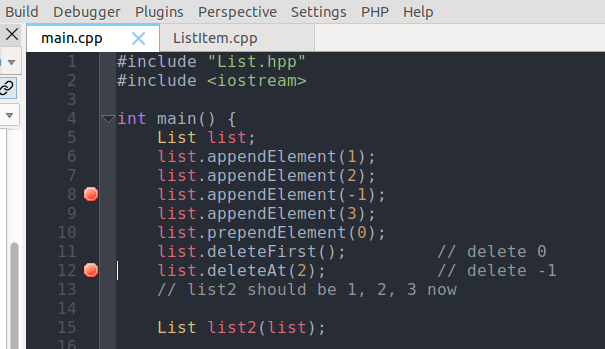
\includegraphics[width=.6\textwidth]{02_memory/figures/breakpoints.png}
	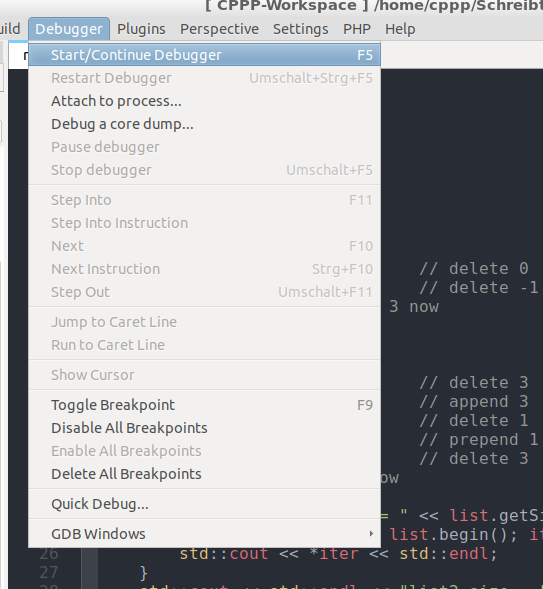
\includegraphics[width=.3\textwidth]{02_memory/figures/start_debugger.png}
	\caption{Setze Breackpoints und starte Debugger}
	\label{fig:breakpoints}
\end{figure}

%\begin{figure}
%	\centering
%	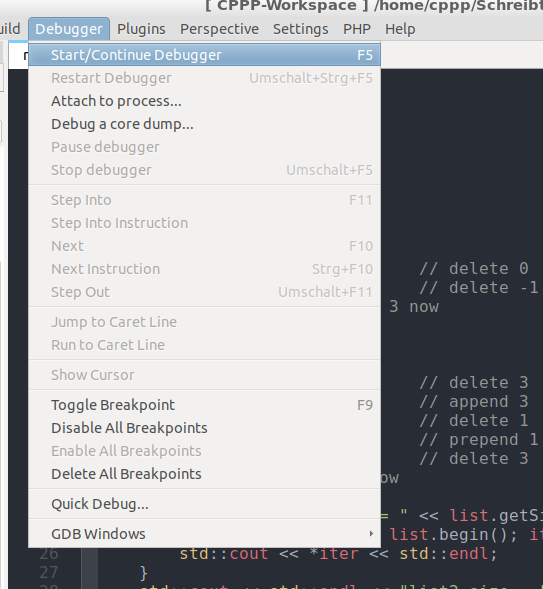
\includegraphics[width=.9\textwidth]{02_memory/figures/start_debugger.png}
%	\caption{Starte den Debugger}
%	\label{fig:start_debugger}
%\end{figure}

\begin{figure}
	\centering
	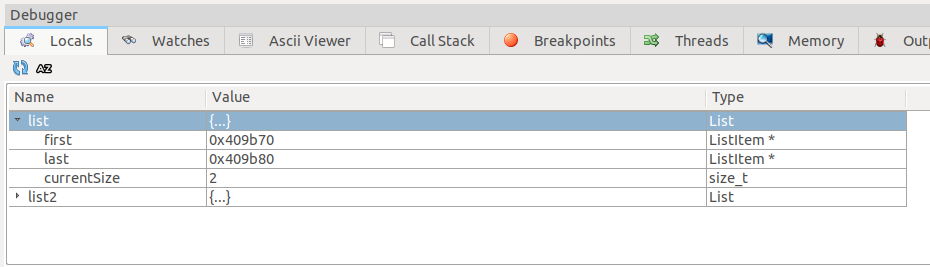
\includegraphics[width=.9\textwidth]{02_memory/figures/locals_view.png}
	\caption{Inspizieren von Variablen}
	\label{fig:locals_view}
\end{figure}

%\begin{figure}
%	\centering
%	
\includegraphics[width=.9\textwidth]{02_memory/figures/debugtools.png}
%	\caption{Debug Werkzeuge: }
%	\label{fig:debug_tools}
%\end{figure}

\hints{
	\item Mit step in kannst du auch die Aufrufe sehen, welche im For-Schleifenkopf gemacht werden.
}
\newpage
\section{Exceptions}
Ähnlich wie in Java können Fehler während der Programmlaufzeit in C++ mittels Exceptions signalisiert werden.

\lstinputlisting{problems/listings/exceptions_intro.cpp}

Es gibt jedoch einige Unterschiede zur Fehlerbehandlung in Java.
Das aus Java bekannte \lstinline{finally}-Konstrukt existiert in C++ nicht.
Außerdem kann jede Art von Wert geworfen werden -- sowohl Objekte als auch primitive Werte wie z.B. \lstinline{int}.
In der Praxis wird es jedoch empfohlen, den geworfenen Wert von \lstinline{std::exception} abzuleiten oder eine der existierenden Klassen aus der Standardbibliothek zu nutzen.

Im Gegensatz zu Java kann man Objekte nicht nur \emph{by-Reference} sondern auch \emph{by-Value} werfen und fangen.
In diesem Fall wird das geworfene Objekt nach der Behandlung im \lstinline{catch}-Block automatisch zerstört.
Wenn es \emph{by-Value} gefangen wird, wird das geworfene Objekt kopiert, ähnlich wie bei einem Funktionsaufruf.
Beispiel:

\lstinputlisting{problems/listings/exceptions_by_what.cpp}

In der Praxis hat es sich durchgesetzt, \emph{by-Value} zu werfen und \emph{by-const-Reference} zu fangen.

\subsection{Implementierung einer Dummy-Klasse}
Erstelle eine Klasse \lstinline{C} und implementiere einen Konstruktor, einen Copy-Konstruktor und einen Destruktor.
Versehe diese mit Ausgaben auf der Konsole, so dass der Lebenszyklus während der Ausführung ersichtlich wird.

\subsection{}
Experimentiere mit Exceptions.
Probiere insbesondere die beiden o.g. Fälle aus und beobachte die Ausgabe.
Wann wird ein Objekt erstellt/kopiert/gelöscht?
Teste auch, was passiert, wenn du mehrere \lstinline{catch}-Blöcke erstellst und sich diese nur in der Übergabe unterscheiden (Wert/Referenz).

\lstinputlisting{problems/listings/exceptions_multiple_catch.cpp}

Welcher \lstinline{catch} Block wird aufgerufen?
Spielt die Reihenfolge eine Rolle?

\subsection{Erweitern der Klasse \lstinline{List}}
Füge der Klasse \lstinline{List} vom Vortag Bereichsprüfungen hinzu.
Schreibe die Methoden \lstinline{insertElementAt()}, \lstinline{getNthElement()} und \lstinline{deleteAt()} so um, dass eine Exception geworfen wird, falls der angegebene Index die Größe der Liste überschreitet.
Verwende als Exception die Klasse \lstinline{std::out_of_range}\footnote{\url{http://en.cppreference.com/w/cpp/error/out_of_range}} aus dem \lstinline{stdexcept} Header.

\hints{
    \item Du musst hierbei keinerlei \lstinline{catch} Block verwenden, da es rein um das werfen einer Exception geht.
}

\subsection{Testen der Implementierung}
Teste die erweiterte Implementierung der Klasse List.
Provoziere eine Exception, indem du falsche Indices angibst, und fange die Exception als \lstinline{const} Referenz mit einem \lstinline{catch} Block ab (s.o.).
Du kannst die Methode \lstinline{what()}\footnote{\url{http://en.cppreference.com/w/cpp/error/exception/what}} benutzen, um an den Nachrichtentext der Exception zu gelangen.

\newpage
\section{Smart Pointers}
In dieser Aufgabe werden wir uns mit der Benutzung von Smart Pointers vertraut machen. Dazu werden wir die Smart Pointer Klassen \texttt{boost::shared\_ptr} und \texttt{boost::weak\_ptr} der Boost-Bibliothek verwenden.

\subsection{}
Erstellen eine Klasse \texttt{TreeNode}, die einen Knoten eines Binärbaums darstellt.
Jeder Knoten hat einen Inhalt vom Typ \texttt{int} sowie einen Zeiger auf seine beiden Kindknoten.
Statt \glqq roher\grqq{} Zeiger verwenden wir Smart Pointers, die das Speichermanagement übernehmen.
Dadurch wird es nicht nötig sein, Kindknoten manuell zu löschen.
Sie werden automatisch entfernt, sobald der Wurzelknoten gelöscht ist und keine Zeiger mehr auf den Kindknoten zeigen.

\begin{lstlisting}
#include <boost/shared_ptr.hpp>
class TreeNode;

typedef boost::shared_ptr<TreeNode> TreeNodePtr;	// typedef for better reading

class TreeNode {
public:
	/** create a new tree node and makes it shared */
	static TreeNodePtr createNode(int content, TreeNodePtr left = TreeNodePtr(), TreeNodePtr right = TreeNodePtr());
	~TreeNode();
private:
	TreeNode(int content, TreeNodePtr left, TreeNodePtr right);	// create a tree node
	TreeNodePtr leftChild, rightChild;									// left and right child
	int content;																// node content
};
\end{lstlisting}

Der Konstruktor von \texttt{TreeNode} privat, weil nur die Smart Pointer die Verantwortung für die Lebenszeit eines Objektes übernehmen sollen und bestimmen, wann es gelöscht wird.
Würde man \texttt{TreeNode}-Objekte direkt auf dem Stack anlegen, kann es passieren, dass der Objektdestruktor mehrmals aufgerufen wird -- einmal vom Smart Pointer und einmal beim Verlassen der Funktion.
Ebenso sollten wir keine Rohzeiger auf das Objekt erzeugen, da diese das Speichermanagement der Smart Pointer umgehen.
Stattdessen stellen wir eine statische Methode bereit, um \texttt{TreeNode}-Objekte auf dem Heap zu erzeugen und diese direkt einem Smart Pointer zu übergeben.

Implementiere den Konstruktor, Destruktor sowie \texttt{createNode}.
Der Konstruktor sollte die Attribute entsprechend initialisieren.
Schreibe auch eine Textausgabe, die den Zeitpunkt der Erzeugung eines \texttt{TreeNode}s deutlich macht.
Der Destruktor braucht die Kindknoten nicht zu löschen, da dies bei der Zerstörung des Elternknotens automatisch geschieht.
Füge auch hier eine Textausgabe ein, die die Zerstörung des Objekts sichtbar macht.

Das Schlüsselwort \textbf{static} sowie die Default-Parameter müssen bei der Implementation der Methode ausgelassen werden.
Der Smart Pointer für die Rückgabe wird mit einem Zeiger auf ein \texttt{TreeNode}-Objekt initialisiert. Somit lautet der Methodenrumpf

\begin{lstlisting}
TreeNodePtr TreeNode::createNode(int content, TreeNodePtr left, TreeNodePtr right) {
	return TreeNodePtr(new TreeNode(...));
}
\end{lstlisting}

\subsection{}
Teste, ob die einzelnen Knoten tatsächlich gelöscht werden, sobald kein Zeiger mehr auf den Elternknoten zeigt.
Erstelle dafür einen kleinen Baum:

\begin{lstlisting}
TreeNodePtr node = TreeNode::createNode(1, TreeNode::createNode(2), TreeNode::createNode(3));
\end{lstlisting}

Führe das Programm aus und beobachte die Ausgabe.
Sobald \texttt{main} verlassen wird, wird der Zeiger \texttt{node} gelöscht, und somit auch das dahinterliegende \texttt{TreeNode}-Objekt mit all seinen Kindknoten.

Um ganz sicher zu gehen, dass der Baum tatsächlich beim Löschen des letzten Zeigers zerstört wurde und nicht etwa durch das Beenden des Programms, kannst du \texttt{node} mit einem anderen Baum überschreiben.
Füge in diesem Fall am Ende des Programms eine Textausgabe hinzu, damit ersichtlich wird, dass der erste Baum noch vor Verlassen der \texttt{main} gelöscht wurde.

\subsection{}
Nun wollen wir \texttt{TreeNode} so erweitern, dass jeder Knoten Kenntnisse über seinen Elternknoten besitzt.
Füge das Attribut

\begin{lstlisting}
	TreeNodePtr parent;		// parent node
\end{lstlisting}

hinzu.
Da der Elternknoten beim Erzeugen eines \texttt{TreeNode}s undefiniert ist, brauchst du den Konstruktor nicht zu ändern. \texttt{parent} wird dann automatisch mit NULL initialisiert.

Implementiere die folgende Methode, die einem Knoten seinen Elternknoten zuweist:

\begin{lstlisting}
	void setParent(const TreeNodePtr &p);		// set parent of this node
\end{lstlisting}

\emph{Hinweis}:
\texttt{p} wird in diesem Fall nur deshalb als \texttt{const} Referenz übergeben, da es verhältnismäßig aufwändig ist, einen Smart Pointer zu kopieren.
Beachte, dass im obigen Fall der Smart Pointer selbst const ist, und nicht das Objekt, worauf er zeigt.

Jetzt muss noch \texttt{createNode()} modifiziert werden, sodass \texttt{setParent()} auf den Kindknoten aufgerufen wird. Da ein Smart Pointer die Operatoren $*$ und $->$ überladen hat, lässt er sich syntaktisch wie ein normaler Zeiger benutzen. Um zu überprüfen, ob ein Smart Pointer auf ein Objekt zeigt, kann dieser implizit nach \texttt{bool} gecastet werden. Somit lautet die neue Implementation von \texttt{createNode()}:

\begin{lstlisting}
TreeNodePtr TreeNode::createNode(int content, TreeNodePtr left, TreeNodePtr right) {
	TreeNodePtr node(new TreeNode(content, left, right));
	if (left) {
		left-> ... ; // set parent node
	}
	if (right) {
		right-> ... ; // set parent node
	}
	return node;
}
\end{lstlisting}

\subsection{}
Teste deine Implementation.
Du brauchst dazu in \texttt{main} nichts zu ändern.

Erschreckenderweise siehst du nun, dass überhaupt keine \texttt{TreeNode}-Objekte mehr gelöscht werden.
Die Ursache dafür ist die zirkuläre Abhängigkeit zwischen Kind- und Elternknoten.
Denn selbst wenn sie keine Zeiger auf den Wurzelknoten eines Baumes haben, verweisen die Kindknoten noch immer darauf.

Um dieses Problem zu lösen, müssen die Verweise zum Elternknoten \emph{schwach} (weak) sein.
Ein Knoten darf gelöscht werden, wenn nur noch schwache Zeiger (oder keine) auf ihn verweisen.
Binde dazu den Header \texttt{boost/weak\_ptr.hpp} ein und erstelle ein neues \texttt{typedef} für einen schwachen \texttt{TreeNode} Smart Pointer:

\begin{lstlisting}
typedef boost::weak_ptr<TreeNode> TreeNodeWeakPtr;
\end{lstlisting}

Ändere nun den Typ von \texttt{parent} auf \texttt{TreeNodeWeakPtr}.
Es müssen keine weiteren Änderungen gemacht werden, da starke Zeiger (\texttt{shared\_ptr}) implizit in schwache Zeiger (\texttt{weak\_ptr}) umgewandelt werden können.

\subsection{}
Teste deine Implementation.
Nun sollte sich \texttt{TreeNode} wie gewünscht verhalten.


\cclicense

\end{document}
